\chapter{Konzeption der Anwendung}
\thispagestyle{fancy}

\section{Generelle Struktur der Anwendung}
Zu Beginn gilt es, die verschiedenen Bereiche der Gestaltung zu definieren, die die fertiggestellte Anwendung behandeln soll. Innerhalb des Praxisprojektes wurden verschiedene Themengebiete behandelt, die an dieser Stelle erneut auf eine Umsetzbarkeit hin validiert werden müssen. Die im Praxisprojekt definierten Themengebiete sind:

\begin{itemize}
  \item Typographie
  \item Layout \& Struktur
  \item Whitespace
  \item Farben
  \item Bilder
  \item Interaktive Elemente
\end{itemize}

Der Bereich \textit{Whitespace} konnte schnell ausgeschlossen werden, da obgleich seiner Wichtigkeit für eine gute Gestaltung währen des Praxisprojektes keine Konzepte gefunden werden konnten, auf deren Basis eine Umsetzung möglich wäre.\\
Vor der Zielsetzung, nach Abschluss der Arbeit eine Marktfähige (und damit in ihren Features vollständige) Anwendung erstellt zu haben und der gegebenen Zeit von 9 Wochen für die Umsetzung dieser, musste die Liste der zu behandelnden Gebiete noch weiter eingeschränkt werden.\\
Hier wurde sich für die Bereiche \textit{Bilder} und \textit{Interaktive Elemente} entschieden. Die Wahl erfolgte auf einer evaluation der Relevanz der jeweiligen Bereiche für die Grundlagen einer Gestaltung. Der Bereich \textit{Bilder} ist dabei ein eher technischer, der sich auf die korrekte Handhabung von Bildern fokussiert. Der Bereich Interaktive Elemente ist zwar auch für die Grundlagen der Gestaltung von großer Bedeutung, jedoch ist dieser nur für zwei der drei im Praxisprojekt definierten Arten von Artefakten von Bedeutung (Interaktive Elemente kommen in Textdokumenten nicht vor). Hieraus ergibt sich als Liste von Themen für die Umsatzung innerhalb der Abschlussarbeit:

\begin{itemize}
  \item Typographie
  \item Layout \& Struktur
  \item Farben
\end{itemize}

Außerdem sollten für die Anwendung jeweils ein nutzerfreundlicher Einstieg und Ausstieg gefunden werden. Diese wurden im Praxisprojekt nicht explizit ausgearbeitet und fallen somit auch Konzeptionell in den Bereich der Abschlussarbeit und werden später in diesem Kapitel behandelt.
Die finale Struktur der Anwendung für den Rahmen dieser Arbeit sieht also wie folgt aus (der Bereich \textit{Layout \& Struktur} wurde dabei in \textit{Layout \& Grids} umbenannt):

\begin{itemize}
  \item Einstieg
  \item Typographie
  \item Layout \& Grids
  \item Farben
  \item Ausstieg
\end{itemize}

\section{Einstieg in die Anwendung}
Bereits im Praxisprojekt wurde festgestellt, dass es sinnvoll ist, das Zielmedium des Nutzers zu kennen.

\begin{quote}
  Da sich dieses Tool nicht über die plattformspezifischen Richtlinien hinwegsetzen soll, sollte
von Anfang an die Plattform, für die der Nutzer gestaltet, bekannt sein. Die Inhalte des Tools
sollten sich dementsprechend anpassen. \cite{PoplawskiPP}
\end{quote}

Für die Zielgruppe der Studenten wurden hier drei mögliche Zielmedien definiert: Native App, Website und Textdokument. Diese Zielmedien können aber auch in sich noch weitere Unterkategorien aufweisen. So kann ein Textdokument beispielsweise für das Lesen an einem Bildschirm oder das Lesen in gedruckter Form, oder eine Native App für unterschiedliche Betriebssystem mit unterschiedlichen Gestaltungsrichtlinien entworfen werden. Eine komplette Auflistung der möglichen Zielmedien und ihrer Unterkategorien, die für die hier definierten Themengebeite von Bedeutung sind findet sich in Abbildung \ref{fig:intro} auf Seite \pageref{fig:intro}.
Für den weiteren Verlauf dieses Dokumentes sollen die jeweiligen Zielmedien als \textit{scopes} bezeichnet werden.

\begin{figure}[h]
    \centering
    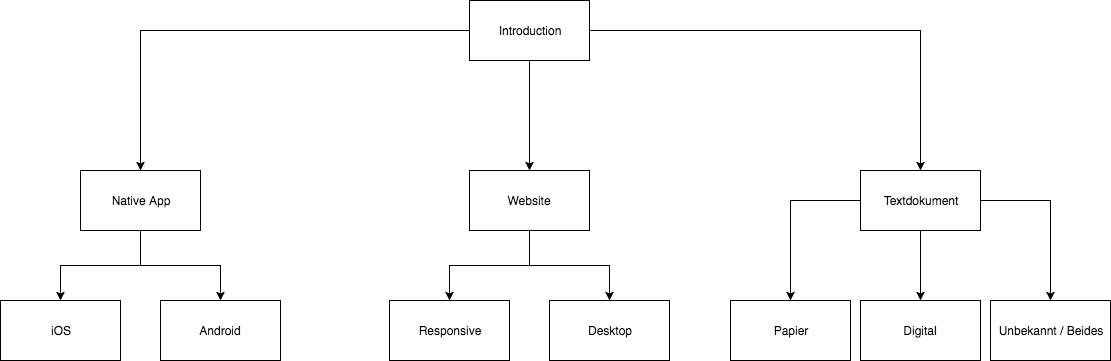
\includegraphics[width=1\textwidth]{images/ablauf_intro.png}
    \caption{Zielmedien der Nutzer und deren Unterkategorien}
    \label{fig:intro}
\end{figure}

Obwohl die Abgrenzung der Bereiche für die hier definierte Zielgruppe ausreichend ist, lassen sich bereits jetzt einige Stellen erkennen, die bei einer möglichen späteren Erweiterung der Zielgruppe überarbeitet werden müsste. Vorrangig betrifft das den Bereich \textit{Website}. Hier ist die vorhandene Unterteilung in \textit{Responnsive} und \textit{Desktop} für ein Echtwelt-Szenario unter Umständen zu allgemein gehalten.

Hier gilt es außerdem festzulegen, wie genau der Nutzer der Anwendung sein jeweiliges Zielmedium mitteilen soll. Ziel muss es dabei sein, die kognitive Arbeit\footnotemark{} diesen so gering wie möglich zu halten. Die in Abbildung \ref{fig:intro} gezeigte Struktur legt hier bereits eine Möglichkeit nahe, dem Nutzer immer nur eine Ebene des Baumes zur gleichen Zeit zu zeigen und so die Zahl der Auswahlmöglichkeiten so gering wie möglich zu halten.\\

\footnotetext{Als kognitive Arbeit werden Prozesse bezeichnet, die ein Nutzer durchführen muss, obwohl diese nicht sein eigentliches Anwendungsziel unterstützen. \cite[S. 410]{Cooper200903}}

Der Nutzer durchläuft einen Wizard\footnotemark{}, der maximal drei Auswahlmöglichkeiten zur gleichen Zeit darstellt. Zur weitern Unterstützung und zur einfacheren Identifizierbarkeit bestehen die Interface-Elemente für die verschiedenen Auswahlmöglichkeiten aus Icon und Text.
Zum Ende des Wizards wird dem Nutzer seine Auswahl noch einmal angezeigt, um so Fehler zu vermeiden, die unter Umständen zu einem späteren Zeitpunkt in der Anwendung den gesamten erarbeiteten Fortschritt nutzlos machen würde.

\footnotetext{"A \textbf{wizard} [...] is an enforced sequence of actions; [...]" \cite[S. 418]{Cooper200903}}

\section{Typographie}
Durch die Umsetzung des Bereiches Typographie als Proof of Concept innerhalb des Praxisprojektes war hier bereits viel grundlegende Konzeptarbeit verrichtet worden, auf der hier aufgebaut werden konnte. Die Grundlegende Interaktion wurde dabei beibehalten: Weiterhin sieht der Nutzer einen Text, der sich auf seine Eingaben hin verändert. Die Eingabe erfolgt weiterhin primär über Schieberegler, die über Tabs gruppiert sind. Die Platzierung dieser beiden Hauptelemente wurde aber verändert, sodass diese jetzt nebeneinander angeordnet sind, und nicht übereinander (vgl. Abbildung \ref{fig:vgl_poc_ba}). Das hat den Vorteil, dass der Nutzer weniger Scrollen muss und so die Möglichkeit hat, den Text und die Bedienelemente gleichzeitig zu sehen.\\
Eine weiter Verbesserung konnte im Bereich der Fehleranzeige vorgenommen werden: Hier wird über ein Icon in der Tab-Navigation deutlich gemacht, dass in einem bestimmten Bereich ein Fehler vorliegt.

\begin{figure}[h]
    \centering
    \includegraphics[width=1\textwidth]{images/vergleich_PoC_BA.png}
    \caption{Der Bereich Typographie, im Praxisprojekt und der Abschlussarbeit}
    \label{fig:vgl_poc_ba}
\end{figure}

Einen weiteren Ansatz stellt die direkte Interaktion mit Elementen dar. So bestünde beispielsweise die Möglichkeit, eine Überschrift anzuklicken und deren Attribute daraufhin direkt zu editieren. Hier wird, im Vergleich zur Interaktion mit Tab-Navigation und Schiebereglern, schneller deutlich, auf welches Element die gewählt Veränderung wirkt, jedoch bietet dieser Ansatz auch einige Nachteile. So können sich Elemente überschneiden (beispielsweise bei der Änderung der Breite des Textes und der Veränderung eines Textabsatzes), wodurch eine genaue Auswahl schwierig wird. Weiterhin ist diese Art der Interaktion nicht sehr verbreitet und würd eine Erklärung benötigen.\\
Um diese Probleme zu umgehen und allgemeine Einstellungen wie die Textfarbe oder die Schriftfamilie festzulegen, wäre also eine Vermischung der beiden Ansätze nötig. Weiterhin ergeben sich Probleme bei einer übersichtlichen Fehleranzeige: Es stellt sich als kompliziert dar, deutlich zu machen, zu welchem Attribut ein Fehler zugehörig ist.\\

Eine Konzeptuelle Neuerung stellt der Reset-Button dar. Dieser erlaubt ein einfaches zurücksetzen auf die Standardeinstellung und nimmt es dem Nutzer damit ab, im Zweifel 10 oder mehr Werte verändern zu müssen, um auf eine bestimmte Einstellung zurück zu kommen.\\
Im Bezug auf die Standardeinstellungen stellt sich die Frage, welche Einstellungen hier zu verwenden sind. Es wurde sich bewusst gegen eine fehlerfreie Standardeinstellung entschieden, da es dem Nutzer nicht möglich ist, in der Anwendung einen Schritt vorwärts zu gehen, wenn noch Warnungen angezeigt werden. So kann sicher gestellt werden, dass der Nutzer sich auf jeden Fall mit dem Bereich Typographie befasst.\\
Auf der anderen Seite sollten die Standardeinstellung nicht zu viele Fehler enthalten, um den Nutzer nicht zu demotivieren. Hier wurde nur ein einziger Fehlerhafter Wert gewählt, der im ersten Tab zu sehen und somit schnell zu beheben ist.\\

\section{Farben}
Während des Praxisprojektes wurde auch hier bereits ein grundlegendes Konzept aufgestellt. Die wichtigsten Punkte, in wenigen Sätzen zusammen gefasst, sind dabei:
Die Farbfindung geschieht in zwei Schritten, das finden der Grundfarbe und das Finden der Akzentfarbe. Farben sollen dabei auch nach Emotionen oder Adjektiven wählbar sein. Für die Betriebssysteme iOS und Android bestehen dabei gesonderte Regeln. \cite{PoplawskiPP}

Im ersten Schritt wurden die verschiedenen Darstellungen für die unterschiedlichen \textit{scopes} festgelegt.

\begin{itemize}
  \item \textbf{Finden einer Grundfarbe:} Hier wurde das Konzept aus dem Praxisprojekt übernommen. Für den jeweiligen \textit{scope} werden die jeweiligen Farben zu Auswahl gezeigt (wobei für die \textit{scopes} Website und Textdokument mit einem Colorpicker eine größere Auswahl an Farben besteht). Ist der \textit{scope} Android, so werden die Farben mit der Helligkeit 500 angezeigt und nach eine Auswahl durch den Nutzer die Abstufungen 300 und 500 automatisch hinzugefügt, um den Raum für Fehler so gering wie möglich zu halten.
  \item \textbf{Finden einer Akzentfarbe:} Für den \textit{scope} iOS entfällt dieser Schritt, für die beiden anderen Schritte wurde dem Nutzer die Möglichkeit gegeben, über Buttons die Art der Akzentfarbe zu wechseln (im Bereich Android über die Helligkeit, in anderen Bereichen in Form des gewählten Kontrastes).
  \item \textbf{Anzeigen des Farbschemas:} Wie bereits beim Einstieg in die Anwendung soll dem Nutzer am Ende das gesamte Farbschema angezeigt werden, bevor er zum nächsten Schritt in der Anwendung über geht. Dies ist vor allem Nötig, weil der Nutzer während der Erstellung immer nur Teile des gesamten Farbschemas sieht.
\end{itemize}

Die Zuordnung von Farben zu Adjektiven gestaltete sich dabei nicht ganz einfach. So machen viele Quellen, gerade im Bereich Marketing, zwar angaben über die Wirkung von Farben, aber genaue Farbabstufungen (zum Beispiel in Form von HEX- oder RGB-Werten) lassen sich nicht finden.
Ziel der Anwendung muss es aber sein, dem Nutzer einen Konkreten Wert zu geben, mit dem dieser Arbeiten kann. Da die Farbfindung über Adjektive hier vor allem den Zweck hat, das Finden einer Farbe für den Nutzer zu erleichtern, und nicht, die Farbwirkung des Artefakts des Nutzer möglichst auf eine Emotion zu bringen, wurde es hier als annehmbar angesehen, die genauen Farbabstufungen zufällig festzulegen. Konkret wurden aus [Artikel] 27 Adjektive extrahiert, zu denen Farbabstufungen gewählt wurden.

Wert wurde auch darauf gelegt, dem Nutzer die von ihm gewählte Farbe bereits währen der Auswahl in einem möglichen späteren Einsatz zu zeigen. Deswegen verfärbt sich ein großer Teil des Hintergrundes während dieses Schrittes entsprechend der Auswahl des Nutzers. Diese Hintergrundfärbung wird auch bei der Wahl der Akzentfarben beibehalten, wobei die Akzentfarben als keiner Flächen auf der Grundfarbe angezeigt werden, Auch hier soll ein direkter Einblick in die mögliche spätere Verwendung geschaffen werden. Abbildung \ref{fig:colors_bg} zeigt diesen Ansatz im fertigen Produkt.

\begin{figure}[h]
    \centering
    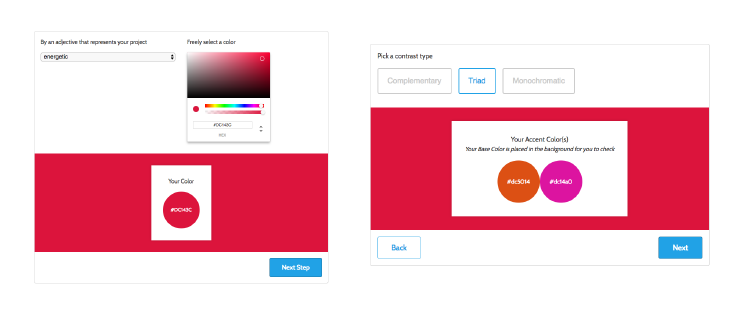
\includegraphics[width=1\textwidth]{images/colors_background.png}
    \caption{Vorschau der ausgewählten Farben in der Anwendung}
    \label{fig:colors_bg}
\end{figure}

\section{Layouts \& Grid}

Auch für den Bereich “Layouts \& Grid” musste weitere, konkrete Konzeptionsarbeit geleitet werden.

Dieser Bereich unterscheidet sich zu den voran gegangenen vor allem dadurch, dass Nutzer mit Verschiedenen Entwicklungzielen hier deutlich verschiedene Interaktionen sehen. Der konkrete Ablauf kann dem Diagramm in Abbildung ZXC entnommen werden. Im folgenden sei der Ablauf anhand der einzelnen Knoten genauer erklärt.

Für Native Geräte ist hier nicht viel Interaktion vorgesehen. Bereits im Praxisprojekt wurde erkannt, dass die Mobilen Plattformen für sich ausreichend genaue Guidlelines in verschiedenen Formen bieten. Im Falle von Android ist in den Material Design Guidelines dabei für verschiedene Elemente sehr genau definiert, wie und mit welchem Abstand diese zu Platzieren sind, im Falle von iOS liefert der Storyboard-Editor von Xcode ausreichend genaue Richtlinien.
Aus diesen Gründen wird hier jeweils auf die Beiden Hilfestellungen hingewiesen und der Nutzer zum nächsten Schritt weiter geleitet.

Für Textdokumente wurde innerhalb des Praxisprojektes bereits eine recht genaue Interaktion konzipiert. Hier sollte es möglich sein, dass der Nutzer den Außenabstand des Dokumentes, ähnlich wie bei der Typographie, selbst verändert und die Anwendung ihm hier Hilfestellungen gibt. Weiterhin sollte die Möglichkeit gegeben werden, den Text in mehrere Spalten aufzuteilen. Diese Interaktion soll auch hier übernommen werden, Abbildung ZXD zeigt ein im Praxisprojekt erarbeitetes Wireframe und ein darauf basierendes, Innerhalt der Abschlussarbeit erstelltes Design.
Hier wurde lediglich die Anordnung verbessert, in dem das Dropdown in einer Reihe mit den anderen Bedienelementen angeordnet ist.
Konzeptionell stellt sich hier außerdem die Frage, ob eine Änderung der Reihenfolge für die verschiedenen Schritte, in der der Nutzer die Anwendung durchläuft für das Erstellen eines Textdokumentes nicht sinnvoll wäre. So könnte hier bereits die Textbreite definiert werden (durch die große des Dokumentes und die Anzahl der Spalten), so dass diese dann im Bereich Typographie fest gesetzt werden kann und der Text besser auf die jeweilige Breite angepasst werden kann.

Für den Bereich Web wurde im Praxisprojekt ein Vergleich verschiedener Grid-Systeme unternommen. Die Ergebnisse dieses Vergleiches sollen auch hier verwendet werden, in dem sie dem Nutzer zum Beispiel in der PDF als Mögliche Grid-Systeme nahe gelegt werden.
Die Anwendung an sich sollte hier aber auch noch einen Versuch unternehmen, den Nutzer an die generelle Arbeit mit Grid-Systemen heran zu führen. Dieser Schritt unterscheidet sich zu den anderen insoweit, dass dieser dem Nutzer kein Konkretes Ergebnis liefern, sondern ihm nur implizites Wissen vermitteln kann.
Der Gedanke hier ist es, den Nutzer mit verschiedenen Einstellungen für Grid-Systeme experimentieren und die Auswirkungen auf eine Seite beobachten zu lassen.

\section{Ergebnisse der Benutzung}
Auch wenn es eines der Hauptziele der Anwendung ist, dem Nutzer während seiner Nutzung interaktiv Wissen zu vermitteln, ist die Anwendung dennoch darauf ausgelegt, den Nutzer bei der Gestaltung eines konkreten Artefaktes zu unterstützen. Hier ist es für den Nutzer hilfreich, auf die von ihm erarbeiteten Ergebnisse auch nach der Verwendung des Tools noch Zugriff zu haben.

Dieser Bereich wurde im Rahmen des Praxisprojektes nicht konzipiert, ist aber für die Wahrnehmung der Anwendung als fertiges Produkt durchaus wichtig. Eine gute Darstellung der Ergebnisse des Nutzers definiert einen ausschlaggebenden Teil der Nutzungserfahrung, da ohne diesen Schritt das Gefühl aufkommen würde, dass während der Zeit der Nutzung kein Mehrwert erwirtschaftet wurde.
Im folgenden sollen also mögliche Darstellungen der Ergebnisse diskutiert und vorrangig die Frage beantwortet werden, welche Darstellungsweise den besten Kompromiss aus Umsetzbarkeit und Mehrwert für den Nutzer bietet.

Die einfachste Darstellung, die in jedem Falle gewählt werden sollte, ist eine transistente Darstellung am Ende eines Nutzung der Anwendung. Hier sollte dem Nutzer noch einmal aufgezeigt werden, welche Werte er innerhalb der Anwendung erarbeitet hat. Transistent ist diese Darstellung, weil diese zunächst nur im JavaScript-Programm im Browser des Nutzers gespeichert wird. Schließt dieser das Browserfenster, so wird auch das JavaScript-Programm beendet und die Ergebnisse gehen verloren.

Ein naheliegender Schritt ist also die Persistierung des Wissens für den Nutzer. Hierfür bieten sich verschiedene Möglichkeiten. \\
Denkbar wäre zum Beispiel das Speichern der Daten als Cookie im Browser des Nutzers. So könnten die Daten beim nächsten Besuch der Anwendung wieder angezeigt werden. Von Nachteil ist hier, dass die Kontrolle über die Speicherung der Daten nicht explizit beim Nutzer liegt: Löscht der Browser den Cookie (zum Beispiel, weil dessen \textit{Max-Age}\footnotemark{} Wert überschritten ist) sind die Daten ohne Eingriffsmöglichkeit des Nutzers verloren.
Eine andere möglichkeit Bietet das Entwicklen eine Backends, das eine entsprechende Datenhaltung verwalten kann. Hier könnten auch meherere Projekte eines Nutzer gespeichert werden. Allerdings liegt der Entwicklungsaufwand für ein solche Backend außerhalb des zeitlichen Rahmens der Abschlussarbeit. \\
Als Kompromiss zwischen Nutzerfreundlichkeit und Entwicklungsaufwand wurde sich für die Persistierung des Wissen in einer Datei im PDF-Format entschieden, die der Nutzer Herunterladen kann.

\footnotetext{Das \textit{Max-Age} Attribut kennzeichnet die maximale Dauer, die ein Cookie im Browser behalten wird. \cite{rfc6265}}

Weitere Verbesserungen der Nutzererfahrung können im Aufbau und Inhalt der Datei erreicht werden. Optimal wäre eine Aufbereitung der Daten, sodass der Nutzer diese möglichst ohne weitere Bearbeitung in seinen Workflow übernehmen kann. Obwohl das Zielmedium des Nutzers bekannt ist, können daraus keine zweifelsfreien Rückschlüsse auf die benötigte Struktur und Form der Daten gezogen werden. \\
So kann beispielsweise bekannt sein, dass der Nutzer eine Webanwendung entwickelt und das Styling für seine Texte in CSS vornimmt. Trotzdem kann der Nutzer zum Beispiel verschieden Preprozessoren wie SCSS, SASS oder LESS verwenden, die alle eine unterschiedliche Syntax verwenden.
Oder es kann bekannt sein, dass der Nutzer an einer Textseite arbeitet, jedoch nicht, welches Textsatzprogramm er verwendet\footnotemark{}.\\
\footnotetext{Ein weiteres Problem stellt die Aufbereitung der Daten für einen Import in ein Textsatzprogramm dar.}
Es ist dabei durchaus Möglich, die benötigten Informationen vom Nutzer zu erhalten und die Daten in Einzelfällen entsprechend aufzubereiten, jedoch liegen auch diese Anforderungen außerhalb des Zeitlichen Rahmens dieser Abschlussarbeit.
